%!TEX root = ./intern_report.tex

\newpage
\subsection{Dive Framework and Wave toolchain}

\subsubsection{Framework Overview}

\paragraph{}
When writing a new design for the DPU, the engineers use an in-house written API called the dive framework for testing and Verification. Due to the sheer complexity of the programs that need to be adapted to run in the DPU, the code is brought down to lower semantic levels step by step using the toolchain which consists of 5 main tools.

\begin{itemize}
    \item Wave C Compiler (WCC) - Compiles the C++ code to a WFG code 
    \item Wave Flow Graph Simulator (WFGsim) - Simulates the flow graph and compares it with the I/O values of the C++ code
    \item Wave Flow Graph Compiler (WFGC) - Compiles the WFG code to a Wave Assembly code
    \item Wave Machine Simulator (WMsim) - Simulates the Wave assembly code in a virtual machine environment
    \item Wave Assembly Compiler (WAsm) - Compiles the assembly code to an encrypted binary file format called Lantana
\end{itemize}


\begin{figure}[h]
    \centering
    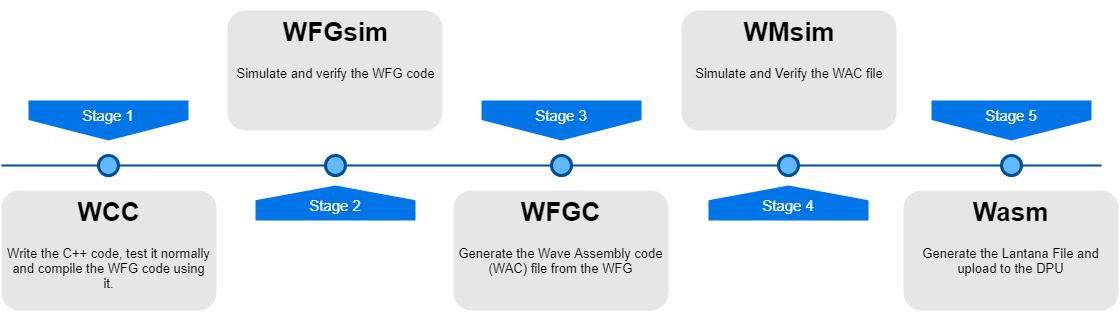
\includegraphics[trim=0cm 0cm 0cm 0cm, clip=true,scale=0.35]{figures/wave_flow.png}
    \caption{Wave Toolchain and design flow\label{Fig:waveflow}}\vspace{-4mm}
    \end{figure}

\subsubsection{Repository Structure}
\paragraph{}
Different cloud folders that contains software code are known as repositories. Wave source codes are stored in five main repositories hosted in a local git server. For better identification, the tools are again divided in to two classes, Wave Front End (WFE) and Wave Back End (WBE). WCC, WFGsim and WFGC belong to the WFE while WMsim and WAsm are contained in the WBE. In the Wave source code, the code for WFE and WBE are stored in separate repositories while the code that is shared by these are stored in a third repository named wcore. Test codes are stored in the wtest repository while experimental tools are stored in the final repository, tools.

\subsubsection{WCC}
\paragraph{}
Wave computing has their own version of C++ dubbed WaveC, which is C++ with added support for data channels and some more things. This language receives constant updates from a team inside wave and thus, developers must build the C language from its source code frequently. This is also true for other tools.

\paragraph{}
WCC uses a technology called LLVM~\cite{LLVM} to convert one human written code in to a different human readable code. It works by analyzing the code and simplifying it to a desired level and assembling the result back together on a predefined syntax. After simplifying the code again and again, the desired output can be obtained, which in this case is the WFG code file.

\subsubsection{WFGsim}
\paragraph{}
This was the most important tool for me since my project could eventually evolve to fully replace this tool. I had to analyze this tool very thoroughly to extract functionality for the Py2WFG simulator (section \ref{sec:py2wfgsim}). 

\paragraph{}
WFGsim works by multi-thread programming on python. It initializes separate threads for DPU sections and host processors. Inside each python thread, a library called boost is used to invoke a linear C++ script. These scripts 'talk' to each other via the python interface and python interface also gives the DPU sections a sense of time by governing the order which operations are executed.